\section{Experiments} \label{sec:experiments} 

\begin{table}[t]
\centering
\caption{Hardware setup during training and experimentation.}
\label{tab:eval:experiment-setup}
\begin{tabularx}{\linewidth} {XX}
    \toprule
    Component & Version \\
    \midrule
     GPU & NVIDIA 4070S \\
        GPU RAM & 12GB \\
        CUDA & 12.8 \\
        GPU driver version & 570.86.16 \\
        CPU & Xeon® E5-2699 v4 \\
        CPU core count & 22 \\
        RAM & 256 GB \\
        Disk bandwidth & 3 GB/s \\
        OS & Ubuntu 22.04 LTS \\
        Python & 3.12 \\
        Linux kernel version & 5.15 \\
        PyTorch version & 2.6.0 \\
        PyTorch seed & 42 \\
    \bottomrule
\end{tabularx}
\end{table}

We design our experiments centered around answering \ref{introduction:mrq}, and evaluating SiMo and CoMo against functional and non-functional requirements. Overall, the experiments support three main findings (MFs):

\begin{enumerate}[label=\textbf{MF\arabic*}]
\item \label{evaluation:mf1} Larger, more complex models do not guarantee better results. CoMo achieved only 4\% better accuracy than the average individual EfficientNet, but consumed six times more energy.
\item \label{evaluation:mf2} SiMo achieves 177 times higher throughput than CoMo. However, this comes at the expense of accuracy: 34.3\% for SiMo compared to 57.8\% for CoMo.
\item \label{evaluation:mf3} CoMo ensemble provides only a slight improvement in accuracy compared to the best individual model, B0: 57.8\% for CoMo, 55.3\% for B0). While in some cases this improvement can be crucial, most of the time this difference is insignificant.
\end{enumerate}

\subsection{Experiment Setup}

 During training and evaluation, we used a single GPU cluster with a commercial-grade GPU - Nvidia 4070S - and ensured that no other components bottlenecked the GPU performance. Our complete hardware and software experiment setup is summarized in \Cref{tab:eval:experiment-setup}. To ensure that the GPU is not bottlenecked by PyTorch dataloader speed, we selected the dataloader number of workers to 8 - during test runs, this number showed the highest performance - and we set memory pinning to true, ensuring that dataloader memory pages are not swapped out by the OS. Other hardware components, having significantly lower cost to rent than GPUs, were over-provisioned to ensure close to 100\% GPU load during training and inference. 
 
 The selected CPU is Xeon® E5-2699 v4 with 22 cores - significantly higher than required by the data-loader - and the selected RAM size is 256. To ensure that I/O operations do not bottleneck the data loader, we selected storage with 3 GB/s bandwidth. We used pre-installed by the cluster provider CUDA 12.8, and the driver version is 570.86.16. For OS, we selected Linux Ubuntu. Both OS and PyTorch were of the latest stable version at the beginning of the project - Ubuntu 22.04 LTS with 5.15 Linux kernel version and PyTorch 2.6.0. To validate the experimental setup, we used the wandb framework, recording all CPU, RAM, and GPU loads and GPU energy metrics. 
 
 Throughout training, we recorded both training and validation loss and accuracy to ensure optimal hyperparameter selection. After training all models, we collected their accuracy metrics using the test dataset split. For reproducibility purposes, we keep PyTorch constant at 42 throughout the experimentation process \ref{FR3}. 

\subsection{Tradeoff analyzed: training resources - model accuracy}\label{sec:experiments:exp1}

\begin{table}[t]
\centering
\caption{Model training performance. TT = training time, MPD = mean power draw.}
\label{tab:eval:power-stuff}
\begin{tabularx}{\linewidth} {XXXX}
    \toprule
    Model & MPD [W] & TT [h] & Accuracy \\
    \midrule
    SiMo  & 155              & 6.70              & 34.37\%             \\
CoMo  & -         & 36.65          & 57.80\%             \\
b0    & 178              & 6.36              & 55.31\%             \\
b1    & 185              & 8.70              & 53.70\%             \\
b2    & 187              & 9.34              & 54.63\%             \\
b3    & 183              & 12.25             & 51.41\%    \\
    \bottomrule
\end{tabularx}
\end{table}

As with many complex classification tasks, object classification presents itself with an inherent trade-off between training costs and model accuracy \cite{DBLP:conf/icml/TanL19}. Inherently, models of increasing complexity pose a challenge to fulfilling the requirement of live and instantaneous predictions \ref{nfr1}. While intricate models (e.g., CoMo), employ multiple components to enhance accuracy, they often require significantly more computational resources in contrast to simpler models such as SiMo. These models demand less computational efficiency but potentially compromise accuracy \ref{nfr2}. Prior work shows that, while ensemble-like models can improve generalization \cite{DBLP:journals/ml/Dietterich00}, their efficiency-to-performance ratio is not always optimal, making model selection a crucial factor in balancing accuracy and computational cost.

With this experiment, we quantify this trade-off by analyzing the relationship between GPU power usage (wattage) and accuracy across five different models: EfficientNet-B0, B1, B2, and B3 components of CoMo, and our SiMo architecture.  For this experiment, we tracked two key metrics during the training process: model performance as final accuracy and training costs as GPU power consumption over time.

The data gathered (\Cref{tab:eval:power-stuff}) from measuring GPU power consumption revealed important efficiency trade-offs. While SiMo had the lowest power draw of 155W, its accuracy (34.4\%) lagged behind all EfficientNet models.

Surprisingly, EfficientNet-B0 boasted the second-highest accuracy (55.3\%) at the second-lowest power draw of 178W \ref{nfr5}, \ref{nfr2}, outperforming B3, which consumed 3\% more energy for nearly twice as long, yet achieving 7\% lower accuracy.

\Cref{fig:exp1:fig6} shows the accuracy per watt for each model. SiMo demonstrates the lowest accuracy-to-efficiency ratio of 0.22\%/W, reflecting its design prioritization of computational resources over performance. Out of all EfficientNets \ref{nfr3}, we identify that B0 yields the best performance-per-energy ratio, with 0.31\%/W. These results demonstrate that larger models do not necessarily guarantee better performance. \Cref{fig:experiment:power-costs} additionally demonstrates GPU power consumption over time for training each model. The total energy consumed is significantly higher for EfficientNets of larger complexity.

\begin{figure}
    \centering
    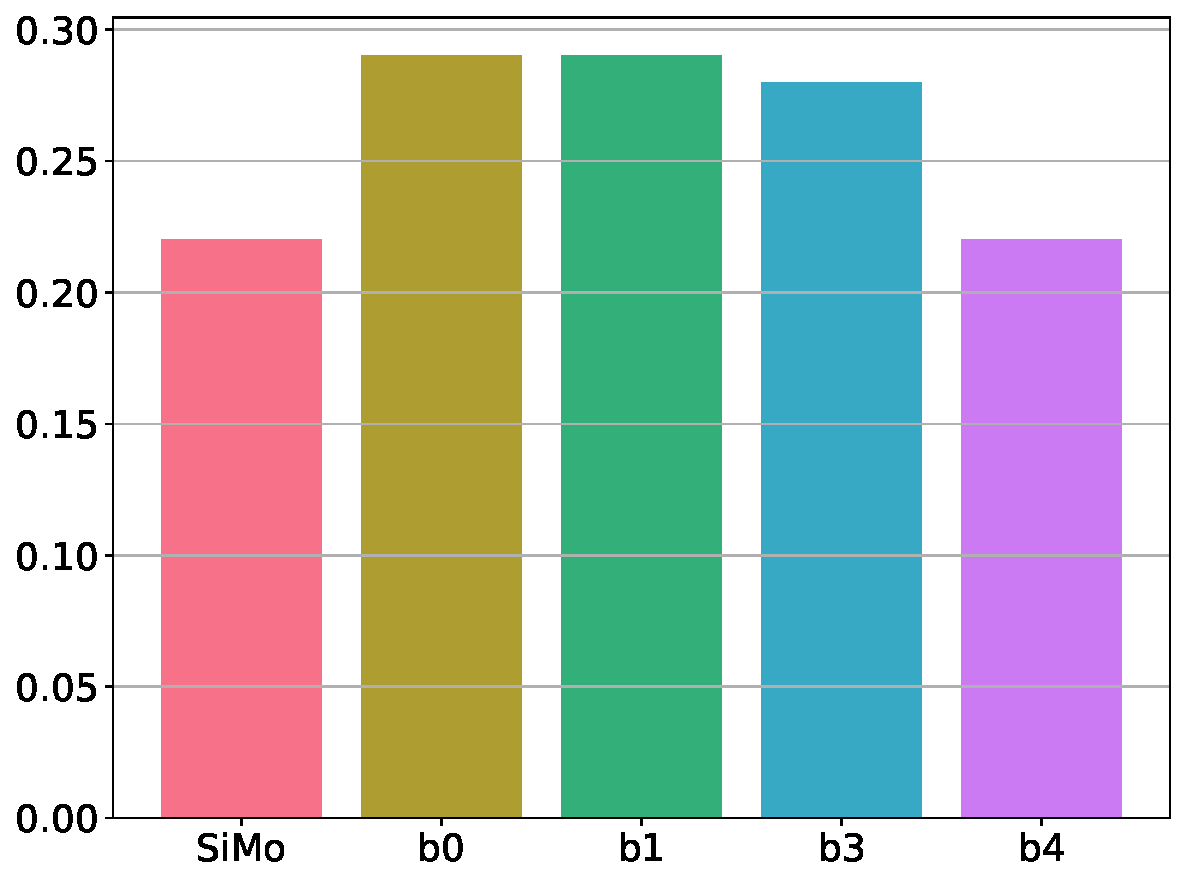
\includegraphics[width=1\linewidth]{figures/accuracy_per_watt.pdf}
    \caption{Accuracy Per Watt.}
    \label{fig:exp1:fig6}
\end{figure}

CoMo’s architecture design proved greedy, consuming around five times more energy than its highest-performing component (EfficientNet-B0) \ref{nfr5} while delivering only a slightly higher accuracy of 57.8\%. The aggregate training costs of 734 watts and 36.6 hours reveal severe inefficiencies when examined next to the underwhelming gains in accuracy compared to simply using one of its component models. This finding demonstrates that a tradeoff between model architectural complexity and model training costs in low-resource environments \ref{nfr5} results in smaller models. CoMo, as its aggregated training cost significantly outweighs its marginal performance benefits. While the theoretical advantage of integrating multiple EfficientNet models suggests enhanced feature extraction and generalization, our results indicate that the efficiency-to-performance trade-off does not justify the increased resource consumption. In particular, EfficientNet-B0 emerges as a notably strong performer, fully adheres to high accuracy requirement \ref{nfr2} with significantly reduced energy demands compared to larger models and the full CoMo architecture.

A main finding from this experiment is that larger, more complex models do not inherently guarantee superior results \ref{nfr2}. Instead, the computational cost must be weighed against the actual gains in accuracy. In this case, CoMo’s inability to significantly outperform its own component models highlights inefficiencies in its design. Future work should investigate whether alternative integration strategies or architectural optimizations could improve the efficiency of this approach, and especially whether different combinations of component models could offer different advantages.
% Additionally, while our analysis shows that a single well-selected model (EfficientNet-B0) can rival more elaborate architectures,
Other complex approaches, designed with more effective fusion strategies or optimized training methodologies, could yield superior performance without incurring excessive computational costs. Exploring these alternative architectures, such as weighted ensembling techniques, dynamic model selection, or adaptive training schedules, could provide insights into achieving a better balance between accuracy and efficiency in large-scale classification tasks.

Overall, our findings suggest that when designing classification models, considerations of training cost and efficiency should be given equal weight alongside performance. This perspective can help inform future research directions, guiding efforts to develop high-performing models that also maintain sustainable computational demands.





% % \usepackage{tabularray}
% \begin{table}
% \centering
% \begin{tblr}{}
% Model & Mean power draw (W) & Time to train (h) & Accuracy          \\
% SiMo  & 155              & 6.70              & 34.37\%             \\
% CoMo  & see b0-3         & see b0-3          & 57.80\%             \\
% b0    & 178              & 6.36              & 55.31\%             \\
% b1    & 185              & 8.70              & 53.70\%             \\
% b2    & 187              & 9.34              & 54.63\%             \\
% b3    & 183              & 12.25             & 51.41\%             
% \end{tblr}
% \end{table}





%Also we need to mention probs in section 4d that we didn't train to the fullest, and here that the accuracy is after training but knowing baselines (efficientnets trained on imagenet) we know that these models can achieve the accuracy of more than 80 percent) But also if we trained till it plateud maybe we fucked something up

\begin{figure*}
    \centering
    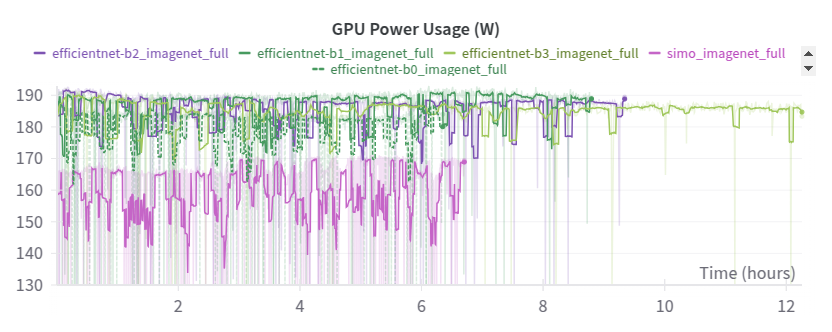
\includegraphics[width=0.95\linewidth]{figures/wattage-graph.png}
    \vspace{-0.3cm}
    \caption{Power costs for model training over time. We provide details for EfficientNet B0, B1, B2, B3, and SiMo.}
    \label{fig:experiment:power-costs}
\end{figure*}


\subsection{Tradeoff analyzed: inference time - model accuracy}\label{sec:experiments:exp2}

% \usepackage{tabularray}

\begin{table}[t]
\centering
\caption{SiMo and CoMo measurements of inference metrics.}
\label{tab:eval:inference-times}
\begin{tabularx}{\linewidth} {XXXX}
    \toprule
    Model & Throughput (samples/sec) & Latency (ms) & Accuracy \\
    \midrule
     SiMo  & 5795.50                  & 4.790        & 34.37\%    \\
CoMo  & 321.63                   & 107.159      & 57.80\%  \\
    \bottomrule
\end{tabularx}
\end{table}


% Paragraph 1 - 100 words
% - what are thoroughput and accuracy?
% - why do we choose those metrics?
% - how do we calculate them?
Throughput and latency are two key performance metrics in evaluating model inference, widely used by the community to quantify system performance. Throughput measures how many samples a model can process per second, reflecting its efficiency in handling large workloads, while latency quantifies the time required to process a single input, making it crucial for real-time applications. We chose these metrics because they provide insight into both the speed and responsiveness of the models. Throughput is calculated as the batch size divided by the inference time, while latency is derived by measuring the total time taken for a single sample.

% Paragraph 2 - 100 words
% - what are the results?
% - what do they suggest?
% - real-world applicability?
% - future research?
The results presented in \Cref{tab:eval:inference-times} indicate a clear trade-off between inference speed and accuracy. SiMo, the simpler model, achieves high throughput (5795.5 samples/sec) and low latency (4.8 ms) but at the cost of accuracy (34.3\%). In contrast, CoMo achieves a significantly higher accuracy (57.8\%) but suffers from lower throughput (321.6 samples/sec) and higher latency (107.2 ms). This tradeoff aligns with our initial hypothesis that the SiMo approach, being optimized for speed, is then more suitable for real-time applications whereas the CoMo approach, prioritizing accuracy, is more applicable in scenarios where precision is the chief concern rather than responsiveness. Future research could explore hybrid approaches that dynamically balance speed and accuracy, potentially adapting model complexity based on real-time constraints.

\subsection{Comparison: CoMo-ensemble against B0-B4}\label{sec:experiments:exp3}
% \usepackage{tabularray}

% Paragraph 1 - 100 words
% - Introduce this experiment
% - Throughput and Latency have already been explained so no need to reiterate
% - but why compare CoMo against its components?
% - what might this tell us?
This experiment investigates how CoMo's accuracy compares to that of its individual components. Given that CoMo aggregates the outputs of multiple EfficientNet models, it is essential to evaluate whether this integration leads to meaningful performance improvements. If CoMo’s accuracy is only comparable to or even lower than that of its best-performing component, it would call into question the benefit of this approach. This comparison helps determine whether the increased computational cost of CoMo is justified or if a simpler model selection strategy would be more effective.

\begin{table}[t]
\centering
\caption{CoMo and sub-component inference measurements.}
\label{tab:eval:como-inference}
\begin{tabularx}{\linewidth} {XXXX}
    \toprule
    Model & Throughput (samples/sec) & Latency (ms) & Accuracy  \\
    \midrule
     CoMo  & 321.63                   & 107.159       & 57.80\% \\
b0    & 2748.30                  & 26.008        & 55.31\% \\
b1    & 1370.84                  & 26.419        & 53.70\% \\
b2    & 1182.51                  & 23.878        & 54.63\% \\
b3    & 1057.22                  & 28.331        & 51.41\%     \\
    \bottomrule
\end{tabularx}
\end{table}


% Paragraph 2 - 100 words
% - what are the results?
% - what do they mean? interpretation
% - is the como approach worth it if its accuracy is only the average of its components? 
The results as shown in \Cref{tab:eval:como-inference} demonstrate that CoMo achieves an accuracy of 57.8\%, which is slightly better than the average accuracy of its individual components. Surprisingly, some individual models, such as b0 (55.3\%), come close to CoMo's performance. CoMo suffers from significantly lower throughput (321.6 samples/sec) and higher latency (107.1 ms) compared to its components. These findings raise the question of whether the CoMo approach is justified if its accuracy does not significantly surpass that of its individual models. The added computational cost may not always be worthwhile unless accuracy gains are more substantial.

% Paragraph 3 - 100 words
% perhaps not - HOWEVER
% our como uses a simple mean between its component's predictions
% other functions might be better
% more complex architectures that take better advantage of component predictions
% etc - FUTURE RESEARCH DIRECTIONS
However, CoMo currently uses a simple mean to combine predictions from its components. More sophisticated aggregation methods—such as weighted averaging, confidence-based selection, or ensemble learning techniques—could potentially improve its accuracy beyond the individual models. Additionally, advanced architectures that better leverage component predictions, such as attention mechanisms or decision fusion strategies, might yield better results. Future research should explore these possibilities to determine whether CoMo can truly surpass its components while minimizing the trade-off in performance.

